\documentclass{beamer}

\usepackage[T1]{fontenc}
\usepackage[utf8]{inputenc}
\usepackage[italian]{babel}
\usepackage{graphicx}
\usepackage{booktabs}
\usepackage{wrapfig}
\usepackage{xargs}
\usepackage{multicol}
\usepackage{minted}
\usepackage{csquotes}
\usepackage{verbatim}

\mode<presentation> {
    \usetheme{Madrid}
    \useoutertheme{infolines} % Alternatively: miniframes, infolines, split
    %\usecolortheme{beamer}
    % \definecolor{myblue}{RGB}{30,108,108}
    \definecolor{myblue}{RGB}{30,108,108}
    \usecolortheme[named=myblue]{structure}
}

\title[Un nuovo modulo di esportazione dati]{\textbf{Ri-progettazione del modulo di esportazione dati del simulatore Alchemist}}

\author{\textbf{Andrea Acampora}}

\institute[] {
    Alma Mater Studiorum $\cdot$ Università di Bologna \\ Campus di Cesena\\
    Dipartimento di Informatica, Scienza e Ingegneria
}

\date{19 Novembre 2021}

\begin{document}

\begin{frame}
  \titlepage
\end{frame}

\begin{frame}{\textbf{Simulazioni computerizzate}}
\begin{block}{Le simulazioni computerizzate sono}
uno strumento molto importante utilizzato nell'analisi del comportamento di sistemi complessi.
\end{block}

\begin{block}{Si compongono delle seguenti fasi}
\begin{itemize}
    \item la presenza di un fenomeno che si intende osservare
    \item l'implementazione di un modello matematico rappresentativo del fenomeno
    \item la trasformazione in un modello eseguibile
    \item l'indagine del fenomeno di partenza attraverso il modello creato
    \item l'analisi delle informazioni ottenute e generate durante la simulazione
\end{itemize}
\end{block}
\end{frame}

\begin{frame}{Generazione di dati tramite simulazioni}
\begin{block}{Le simulazioni}
generano continuamente grandi quantità di dati a prescindere dal contesto in cui operano.
\end{block}
\hfil\hfil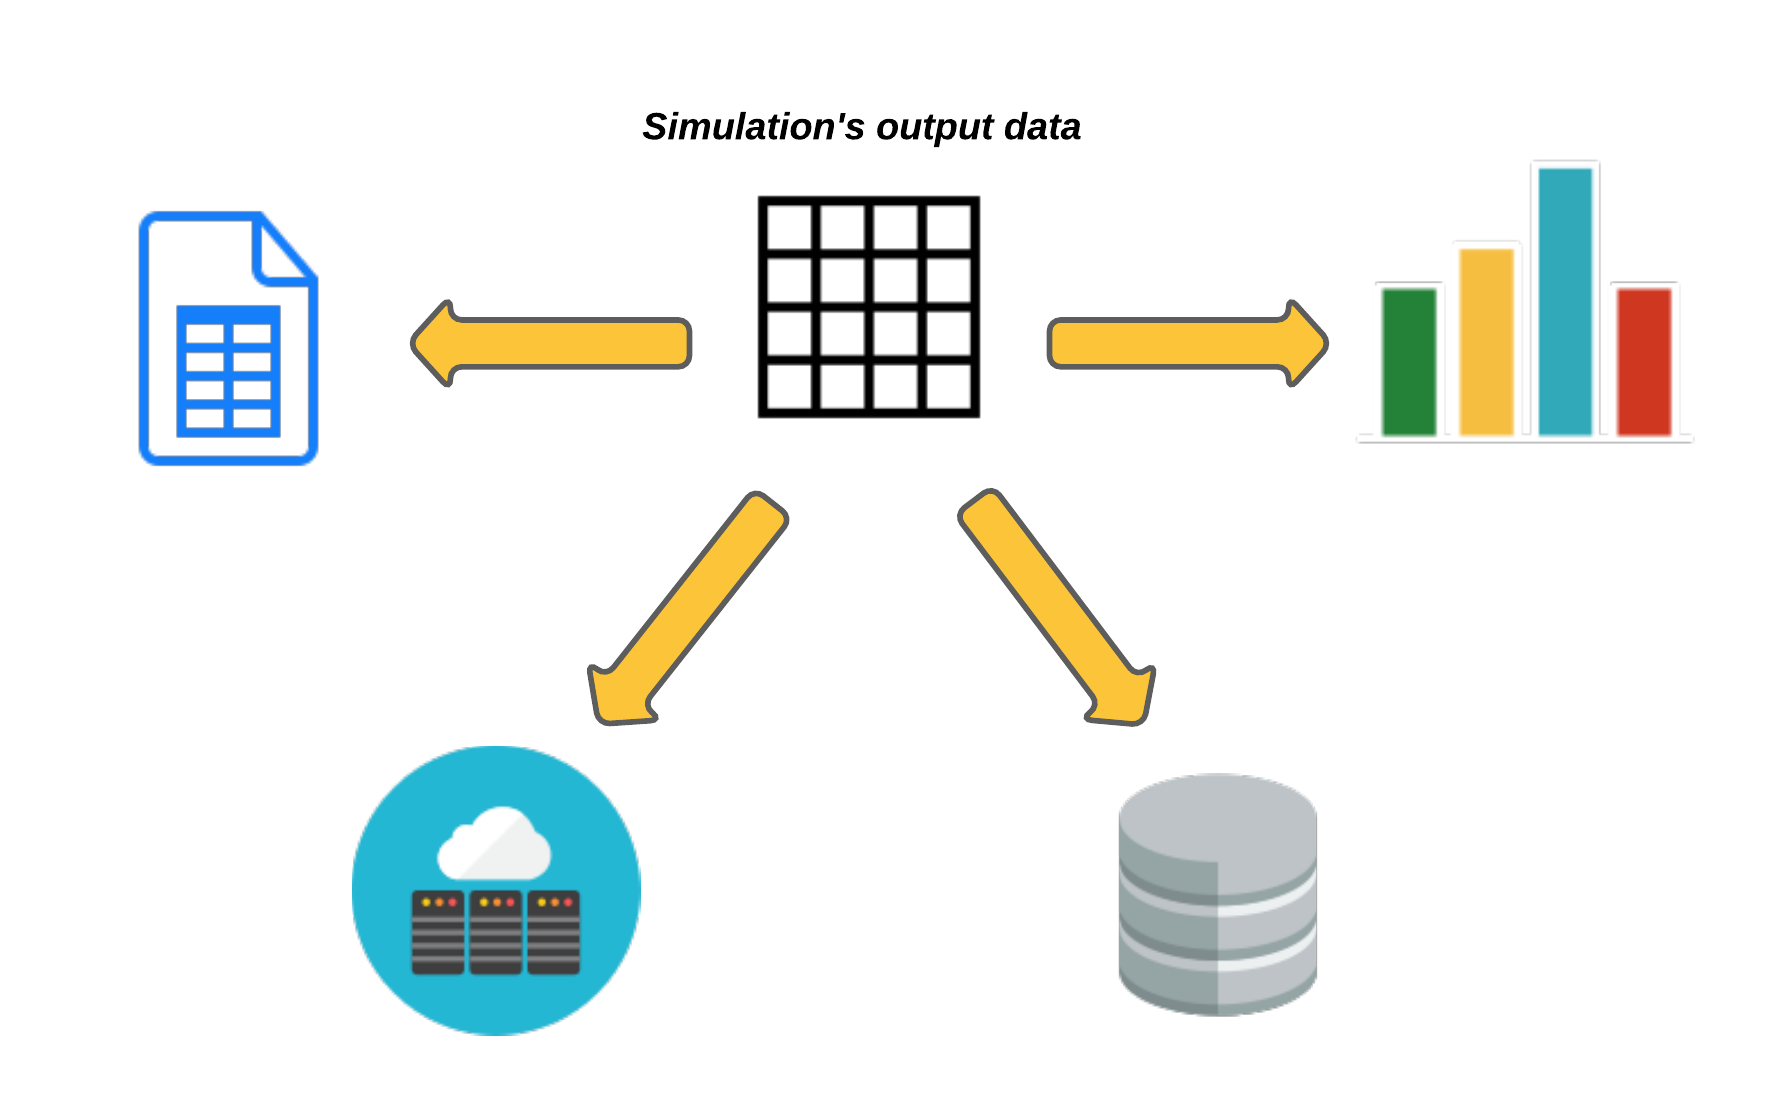
\includegraphics[width=9cm]{images/output_data.png}
\end{frame}

\begin{frame}{\textbf{Alchemist}}
\begin{block}{Alchemist}
è un simulatore stocastico realizzato all'interno dell'Università di Bologna, che permette la simulazione di scenari inerenti la computazione pervasiva, aggregata ed ispirata alla natura.
\end{block}
\begin{block}{Le simulazioni in Alchemist}
vengono configurate all’interno di file YAML, un formato per la serializzazione di dati facilmente leggibile. Nei file di configurazione è necessario specificare quali classi e parametri utilizzare.
\end{block}
\end{frame}

\begin{frame}{Architettura di esportazione dati di Alchemist}
\begin{block}{In Alchemist}
l’attuale sistema di esportazione è basato sulla scrittura dei dati di output su un file di testo in formato CSV.
La scelta dei dati che si intende esportare avviene all’interno del file YAML con la chiave \texttt{export}.
\end{block}
\begin{alertblock}{Problema}
L'esportazione su file di testo, in simulazioni con grandi quantità di dati, presenta diverse criticità tra le quali l'eccessiva dimensione del file generato e la difficoltà nell'accedere ai dati.
\end{alertblock}
\hfil\hfil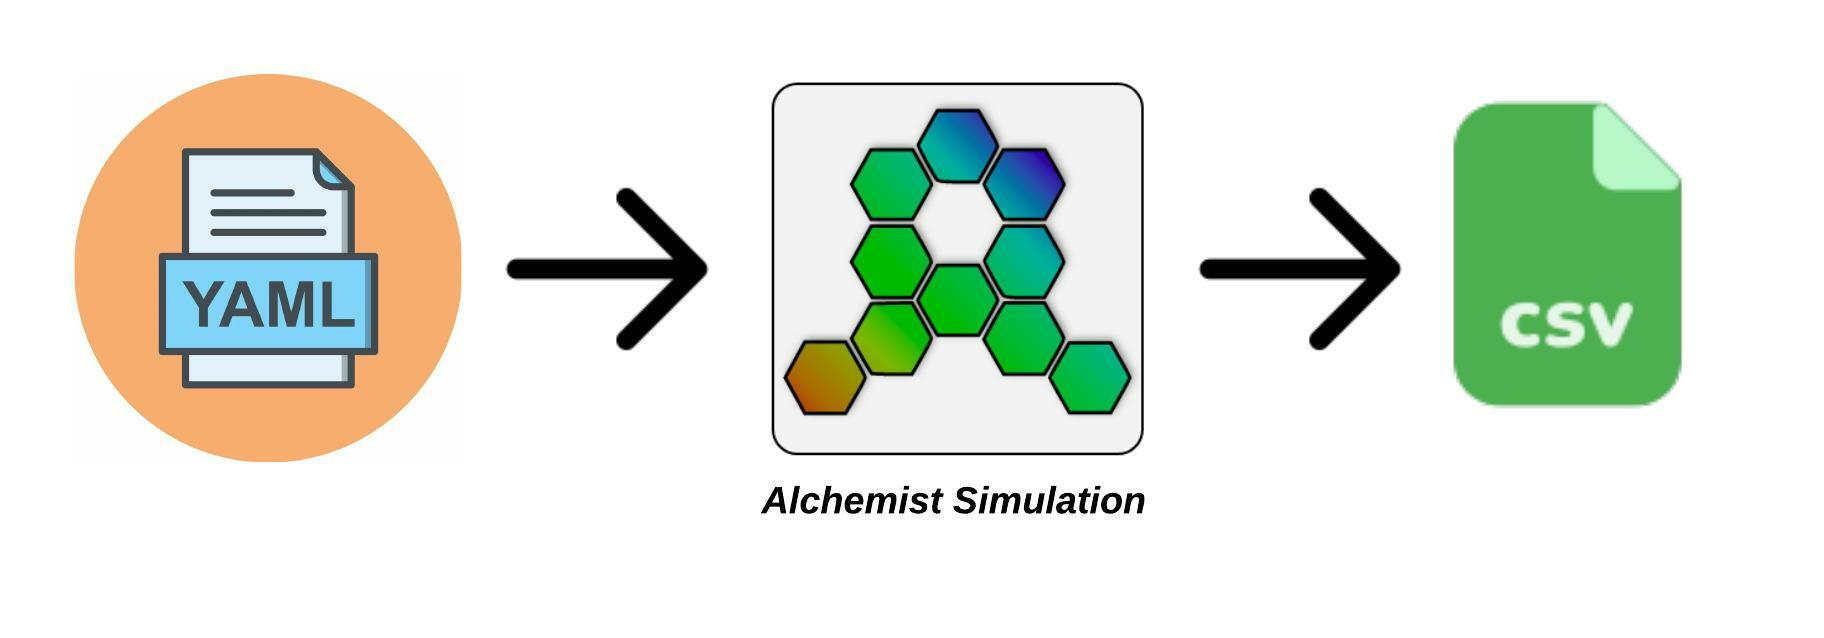
\includegraphics[width=10cm,height=3.5cm]{images/csv-export.jpeg}
\end{frame}

\begin{frame}{Un nuovo modulo di esportazione dati}
\begin{block}{Obiettivo}
Progettazione e sviluppo di un nuovo modulo in grado di esportare i dati
con diverse tecnologie in modo flessibile e dinamico a seconda della configurazione scelta dall’utente.
\end{block}
\begin{block}{Requisiti}
\begin{itemize}
    \item Aumento della flessibilità
    \item Aggiunta di nuovi target per l'esportazione
    \item Aggiunta di esportatori
    \item Configurazione degli esportatori interamente nel file YAML
\end{itemize}
\end{block}
\end{frame}

\begin{frame}{Un nuovo modulo di esportazione dati}
\begin{block}{}
Nel nuovo modulo viene aggiunto un esportatore verso il database \textit{MongoDB}. L’utente può scegliere una tra le varie tecnologie disponibili per esportare dati oppure può scegliere di utilizzarne molteplici contemporaneamente. Inoltre, il nuovo sistema lascia all’utente la libertà di scegliere quali dati assegnare ad ogni tipologia di esportatore.
\end{block}
\hfil\hfil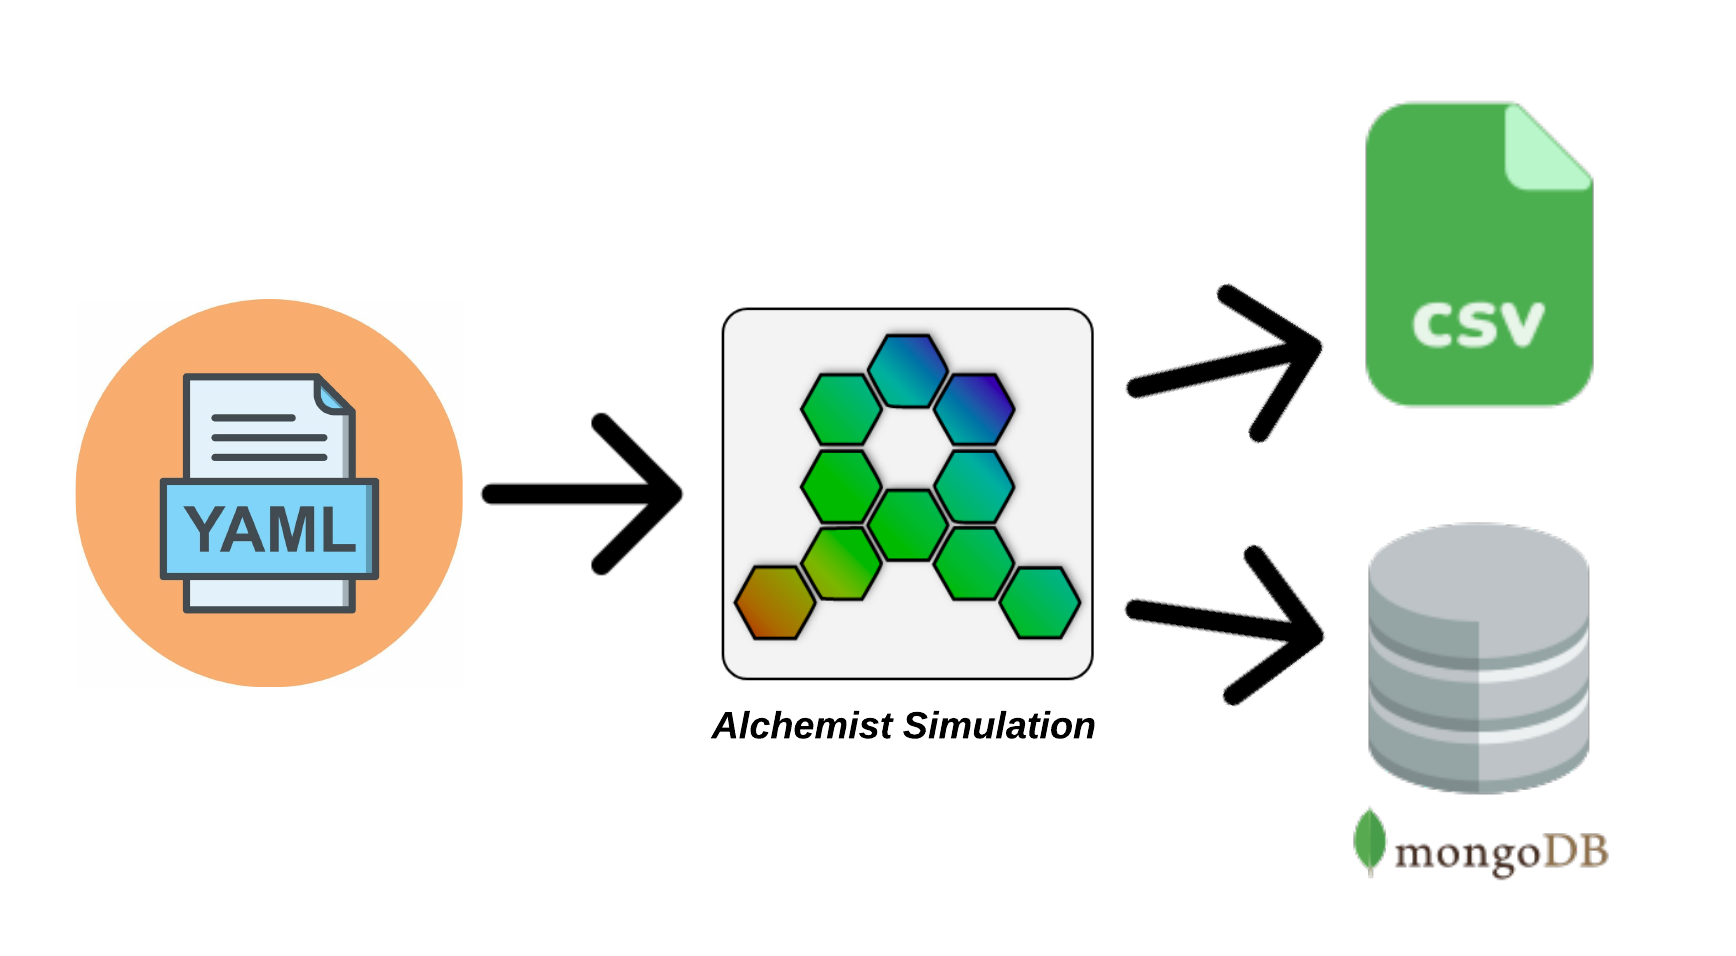
\includegraphics[width=8cm, height=4cm]{images/csv-mongo-export.png}
\end{frame}

\begin{frame}{Un nuovo modulo di esportazione dati}
\hfil\hfil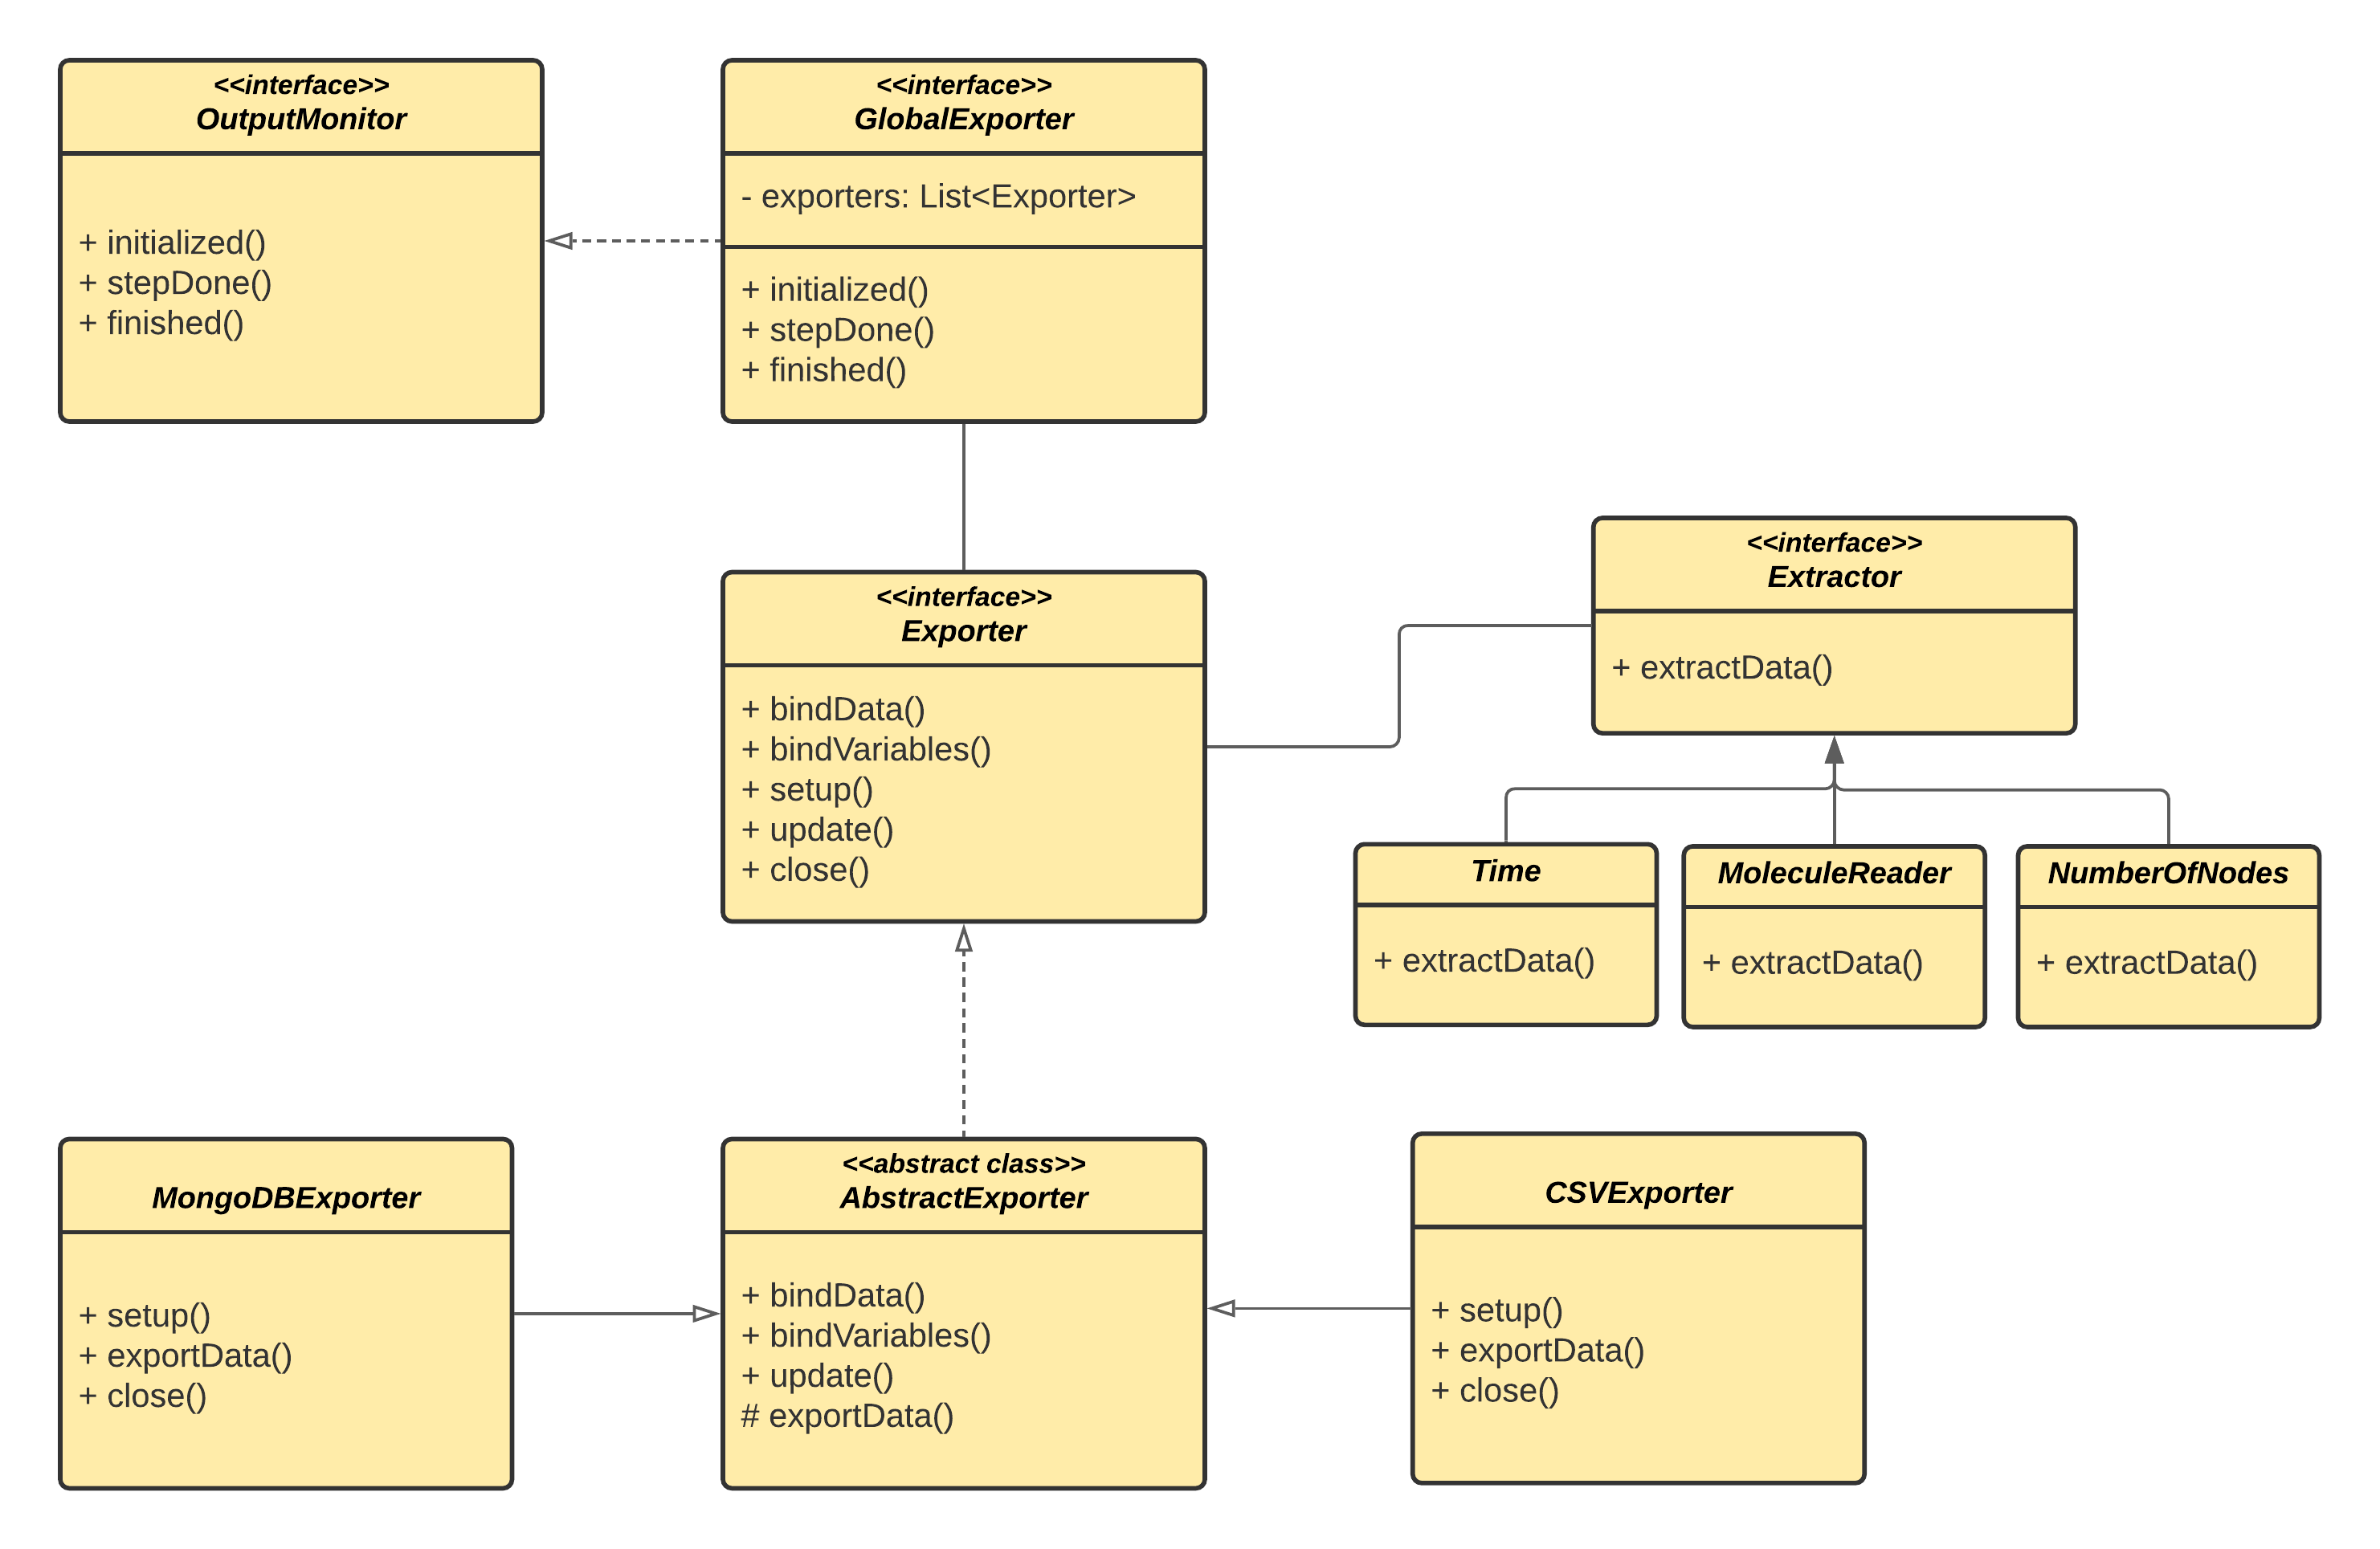
\includegraphics[width=10cm, height=7cm]{images/new_architechture.png}
\end{frame}

\begin{frame}{Valutazione qualitativa}
\hfil\hfil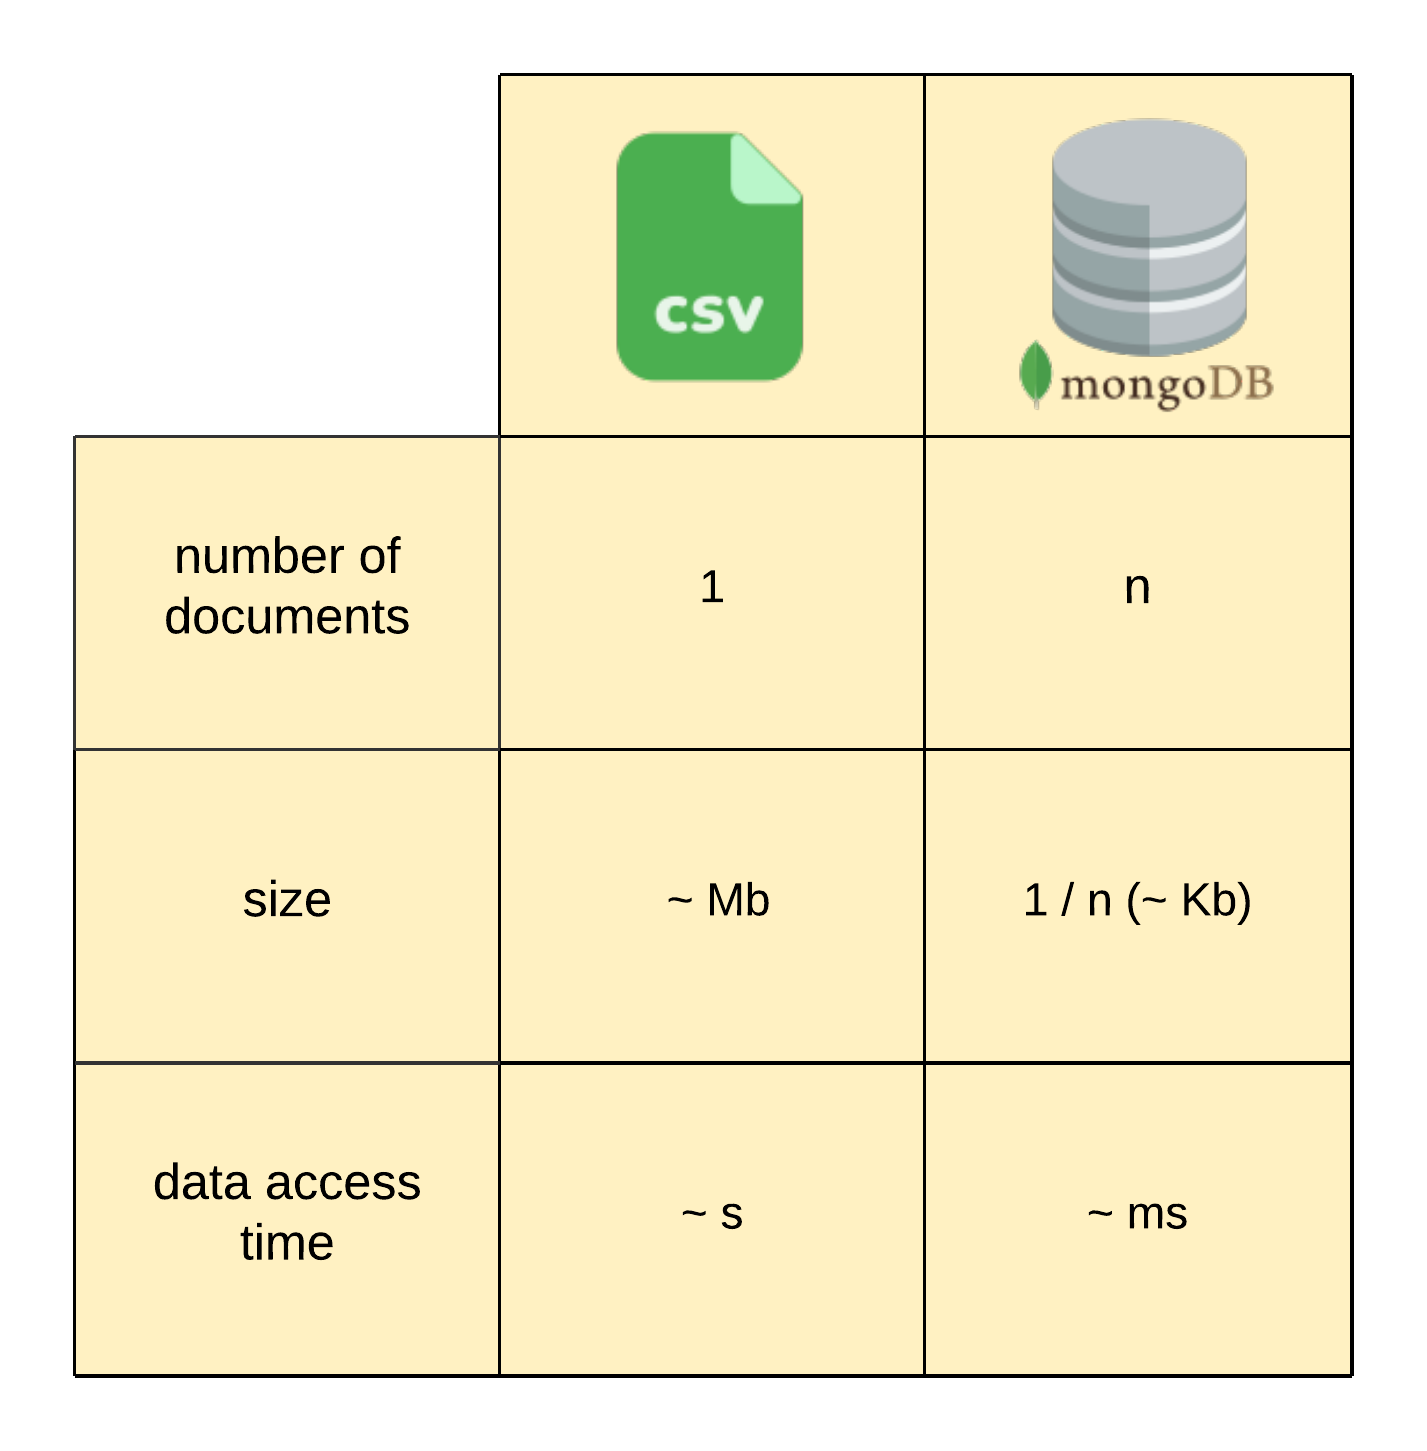
\includegraphics[width=9cm, height=7cm]{images/val_qual.png}
\end{frame}

\begin{frame}{Conclusioni e sviluppi futuri}
\hfil\hfil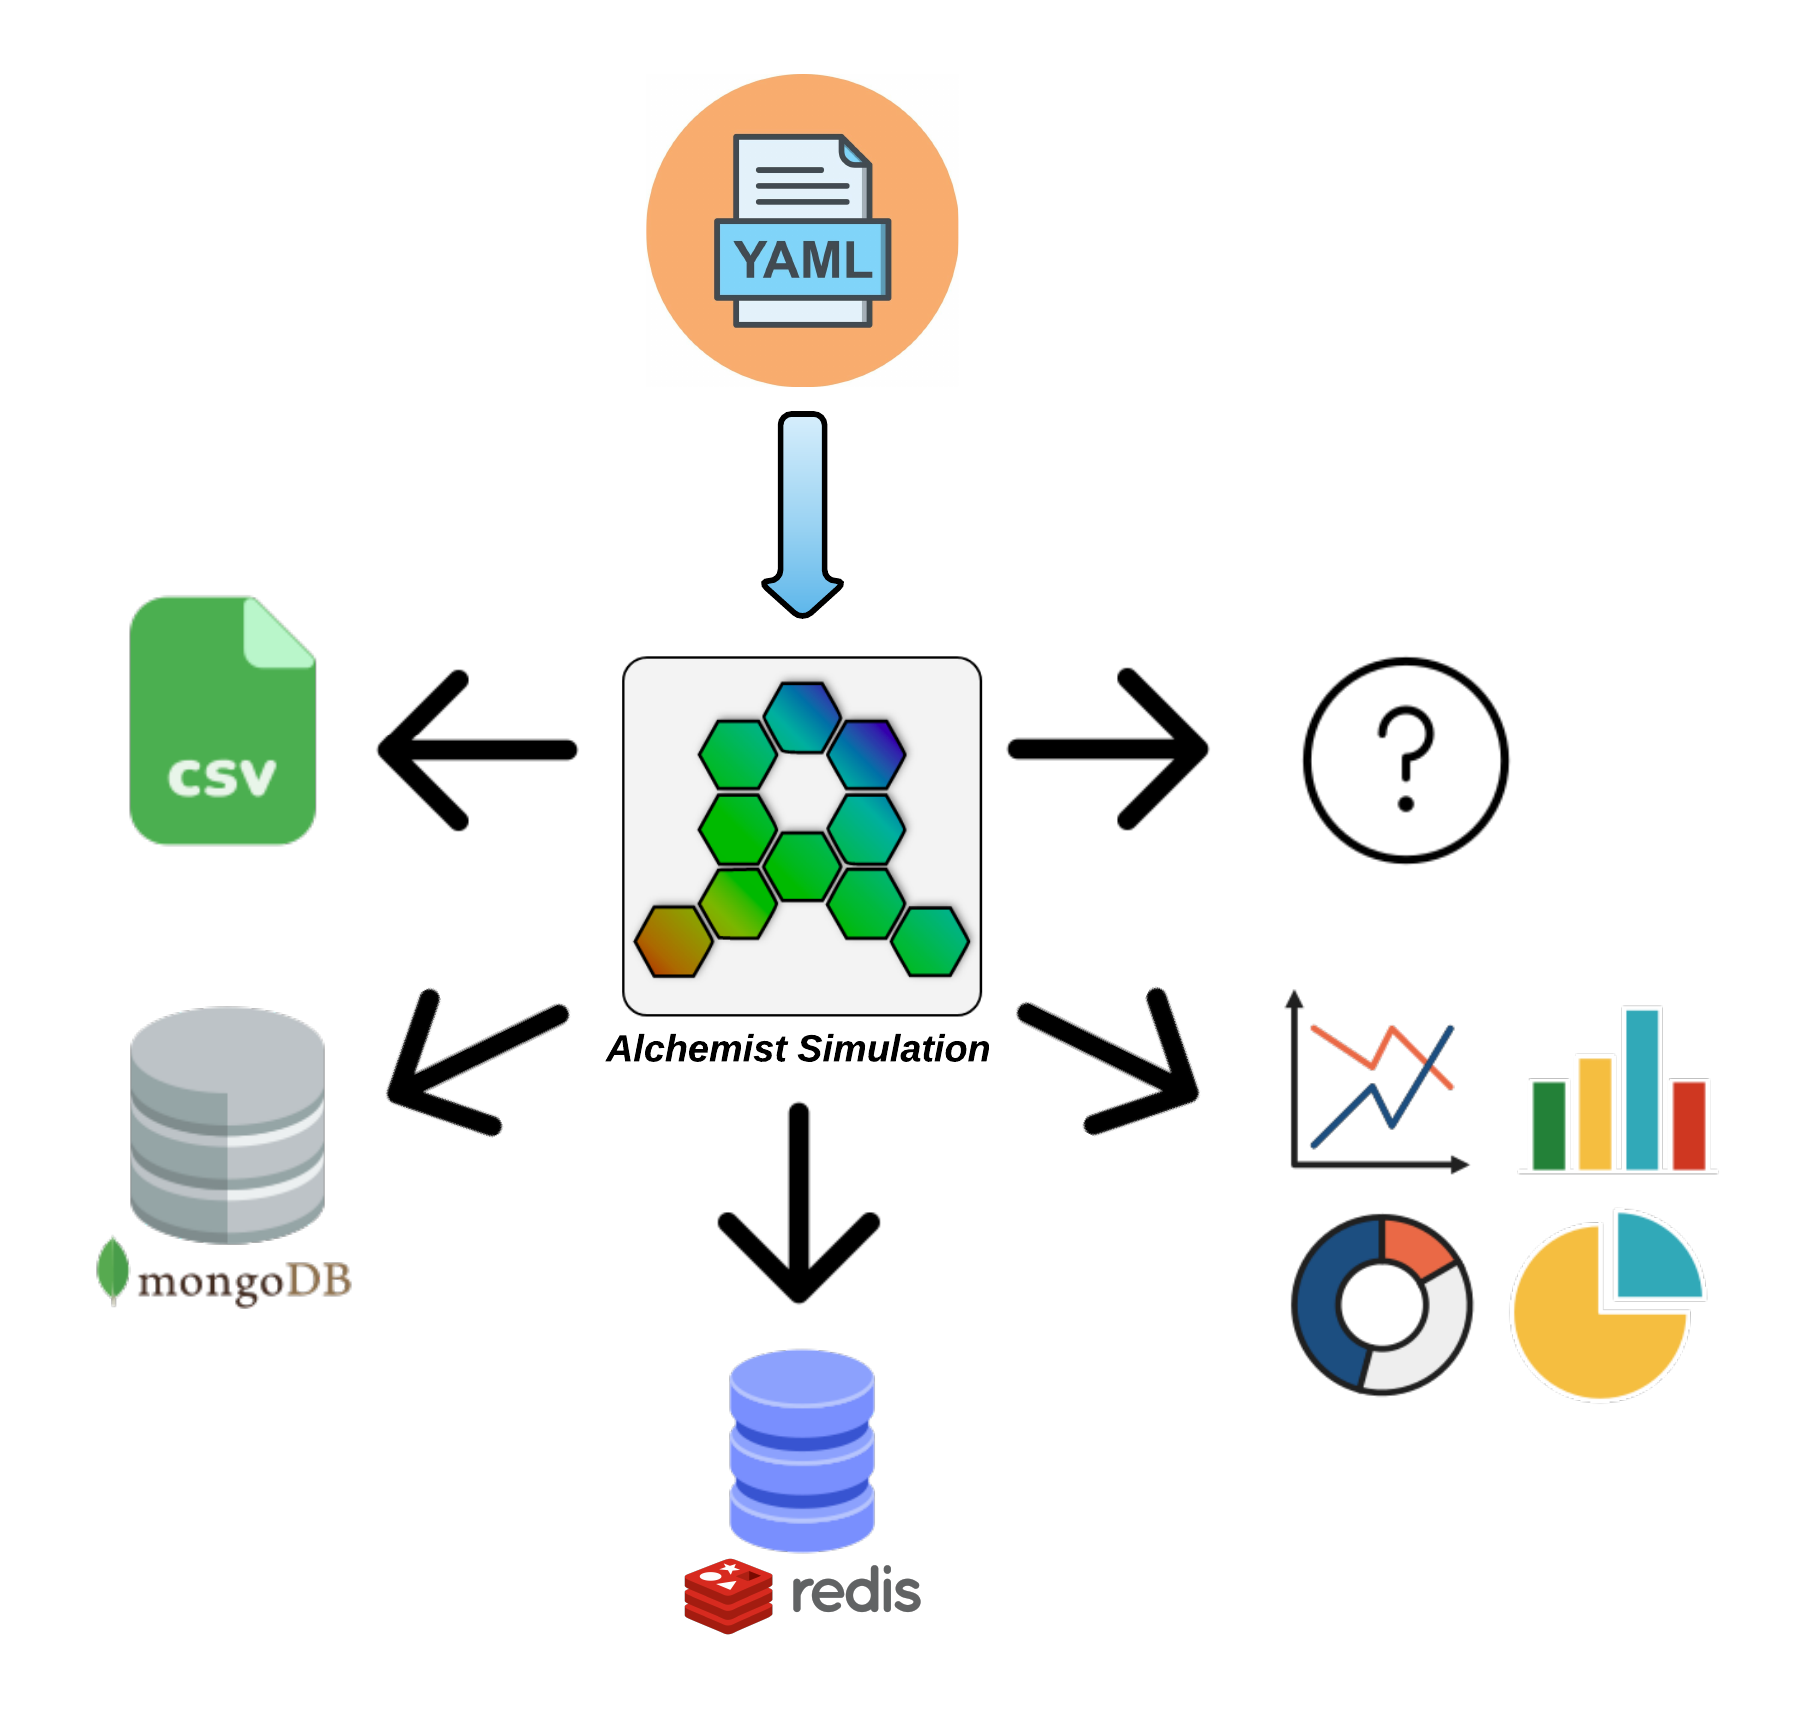
\includegraphics[width=8cm, height=8cm]{images/sviluppi_futuri.png}
\end{frame}

\begin{frame}{\textbf{Riferimenti}}
    \nocite{*}
    \bibliographystyle{unsrt}
    \bibliography{bibliography}
\end{frame}

% \setbeamercolor{background canvas}{bg=myblue}
% \begin{frame}
% \centering
% \color{white} \Huge{\textbf{\textit{GRAZIE}}}
% \end{frame}


\end{document}
